\chapter{Urban Source Identification Results and Discussion}

% https://e-reports-ext.llnl.gov/pdf/312592.pdf they show common false positive isotopes and we see a lot of overlap

This chapter applies machine learning algorithms to solve the problem of identifying a radioactive source in an urban environment. This scenario is applicable when performing source interdiction searching cargo containers, vehicles at boarder crossings, or surveying high profile events. Urban environments present unique challenges to gamma-ray spectroscopy. Background radiation can change over city blocks due to different concentrations of uranium and thorium in building materials. Sources may be purposely shielded by unknown amounts of material to obscure their gamma-ray signal. 

To investigate how simulated parameters affect the performance of dense and convolutional networks with and without autoencoder pretraining, we first determine a sufficient training dataset size for each model and dataset by analyzing their learning curves. We then observe how well each model identifies simulated and measured spectra in a variety of conditions. Finally, we compare the F1 score from our approach with a peak-based Bayesian classifier.

\section{Learning Curve Analysis} \label{sectionlearningcurve}

In this section we analyze learning curves to determine a sufficient number of training dataset examples for the simple and complete networks. Two separate datasets were constructed for this chapter: one using simple dataset parameters, Tables \ref{table:hyperparameter_dataset_easy_parameters}, and the other using complete dataset parameters from Table \ref{table:hyperparameter_dataset_full_parameters}. The datasets included isotopes from the ANSI N42-34-2006 standard, shown in Section \ref{datasets_used_hyperparam_search}. Each dataset contained 1 x 10$^{4}$ randomly generated spectra for each isotope. These datasets will be referred to as the simple and complete master dataset. Models trained on the simple and complete datasets are referred to as simple and complete models.

Different sized training datasets were sampled from both master datasets and trained using each model. This process is illustrated in Figure \ref{fig:learning_curve_training_diagram}. Stratified sampling without replacement was used to sample each master dataset. Stratified sampling keeps the number of isotopes in each sampled subset as equal as possible. Training dataset sizes included 50, 100, 500, 1000, 5000, 10000, 15000, and 20000. For each training dataset size, five sampled subsets of a master dataset were used as training datasets. ANN's were trained using these dataset. A separate holdout validation dataset of 300 spectra (10 examples per class) was used to end training when its F1 score did not improve using an early stopping patience of 10 epochs.

\begin{figure}[H]
	\centering
	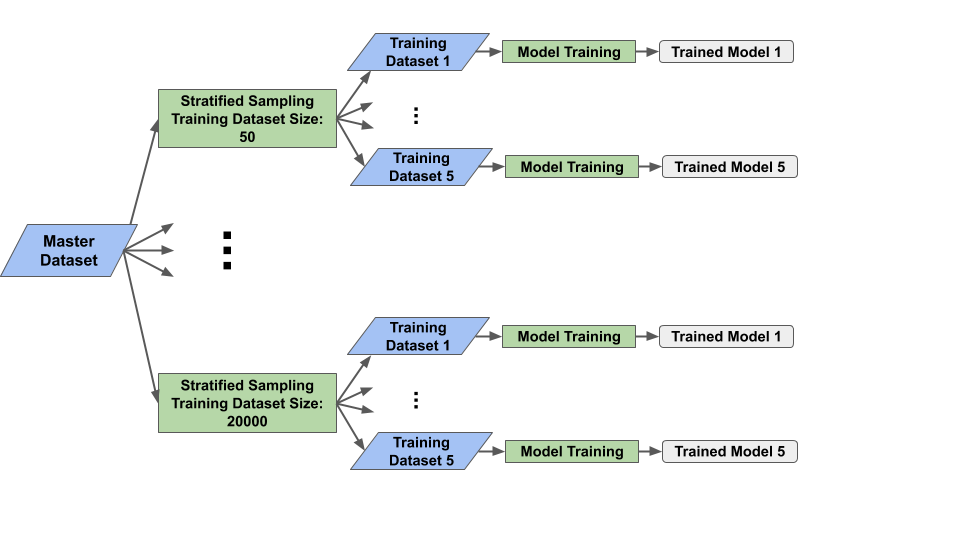
\includegraphics[trim=0 0 0 0,clip,width=1.0\linewidth]{images/learning_curve_training_diagram}
	\caption{Training process used to train models for the learning curves.}
	\label{fig:learning_curve_training_diagram}
\end{figure}

The validation dataset's F1 score was used to construct learning curves for each model. Figure \ref{fig:learning_curves_easy} shows the learning curves for the simple convolutional model's F1 scores reaching an asymptote near one above datasets of 5000 examples. This shows that each convolutional model is well suited to generalize within the simple parameter space. There are no obvious differences between the learning curves for the simple CAE and CNN.

Simple dense models reach an asymptote with a wider variance between F1 scores of 0.8 and 0.9. With fewer than 5000 training examples, the simple DAE had achieved F1 scores lower than the other models. This indicates that the simple DAE did not learn features from the pretraining step. This is likely due to the dense network having an insufficient capacity to reconstruct spectra.


\begin{figure}[H]
	\centering
	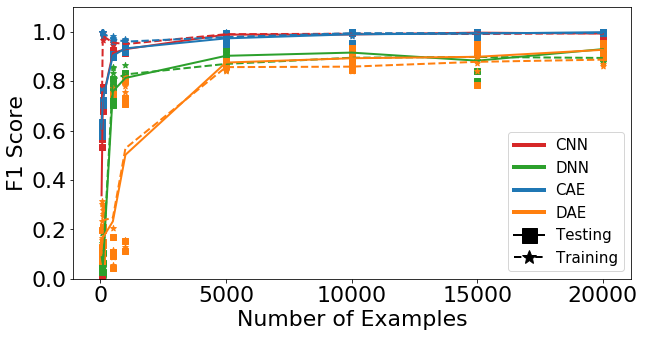
\includegraphics[width=0.9\linewidth]{images/learning_curves_easy}
	\caption{Learning curves for each simple model.}
	\label{fig:learning_curves_easy}
\end{figure}

The validation dataset error curves in Figure \ref{fig:learning_curves_full} are less step than those in the simple learning curve plot. The asymptote for the full dense and convolutional models is also lower than the asymptote for the easy models, demonstrating that the complete dataset is more difficult for the models to generalize to. Even with a comparable number of trainable parameters, the convolutional networks outperform the dense networks. This indicates that the convolutional architecture is better suited to performing gamma-ray spectroscopy. 

\begin{figure}[H]
	\centering
	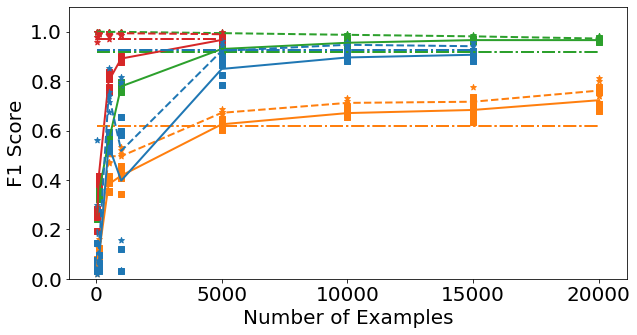
\includegraphics[width=0.9\linewidth]{images/learning_curves_full}
	\caption{Learning curves for each complete model.}
	\label{fig:learning_curves_full}
\end{figure}



\section{Generalization Performance Evaluation}

In this section we analyze each simple and complete ANNs' performance dependence on simulated parameters expected during source interdiction measurements. The process used in this section is outlined in Figure \ref{fig:generalization_performance_diagram}. For each ANN, five models are used as an ensemble by averaging their output, a posterior probability distribution over each isotope. Models trained on a dataset of 10000 examples from Section \ref{sectionlearningcurve} were used in this section.

\begin{figure}[H]
	\centering
	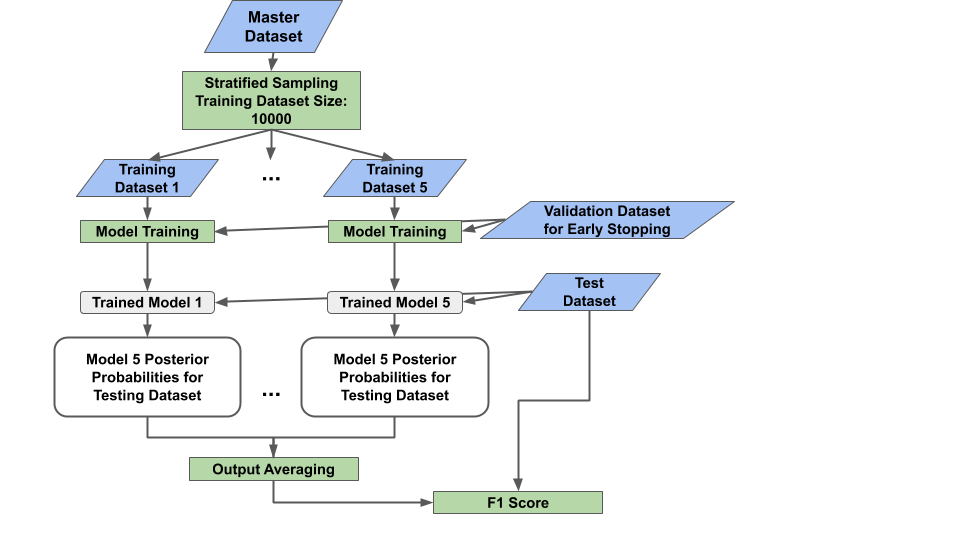
\includegraphics[trim=0 0 210 0,clip,width=1.0\linewidth]{images/generalization_performance_diagram}
	\caption{Model averaging process used to evaluate ANNs using testing datasets.}
	\label{fig:generalization_performance_diagram}
\end{figure}

To compare each ANN's performance, we simulated datasets with various source-detector heights, source-detector distances, detector resolutions, shielding thicknesses, and detector gain calibrations. Datasets were simulated with ten spectra for each ANSI N42-34-2006 isotope and unique parameter. Default simulation parameters for each testing dataset are shown in Table \ref{table:default_sim_params}. Testing datasets were simulated over integration times log-uniformly sampled from one second to an hour and signal to background ratios of 0.1 and 0.5.

\begin{table}[H]
\centering
\caption{Default parameters used for all testing datasets.}
\label{table:default_sim_params}
\begin{tabular}{ll}
% \cline{2-3}
\hline
\textbf{Simulation Parameter} &  \textbf{Value} \\ \hline
Source-Detector Distance [cm] & 175.0\\ 
Source-Detector Height [cm] & 100.0\\ 
FWHM 662 keV [s] & 7.0\\ 
Shielding [\% 200 keV Attenuated] & 0\% \\ 
Calibration - Offset [channels] & 0 \\ 
Calibration - Gain & 1.0 \\ 
Background Counts Per Second & 200 \\ \hline 
\end{tabular}
\end{table}


\subsection{Generalization Performance Dependence on Source-Detector Height}

In this section we analyze how each model's F1 score changes when identifying spectra in datasets simulated with different source-detector heights off the ground. This tests if each model is sensitive to changes in the Compton continuum due to environmental scattering associated with the source-detector height. An example of these changes can be seen in Figure \ref{fig:sim_spectra_height_comparison}. These changes are only noticeably significant in the region below the backscatter peak around 200 keV. This region is important because it contains photopeaks used to detect enriched uranium.

As seen in Figure \ref{fig:sim-generalization-height}, the performance of each network is not significantly changed with changes to source-detector height. This shows that performance is not impacted by the relatively small changes in the continuum caused by varying the source-detector height. Figure \ref{fig:sim-generalization-height} also shows that simple models generalize to changes in source-detector height when the signal-to-background ratio is raised. This shows that the features required to accurately identify low signal-to-background spectra are significantly different from those required by higher signal-to-background spectra. 


\begin{figure}[H]
	\centering
	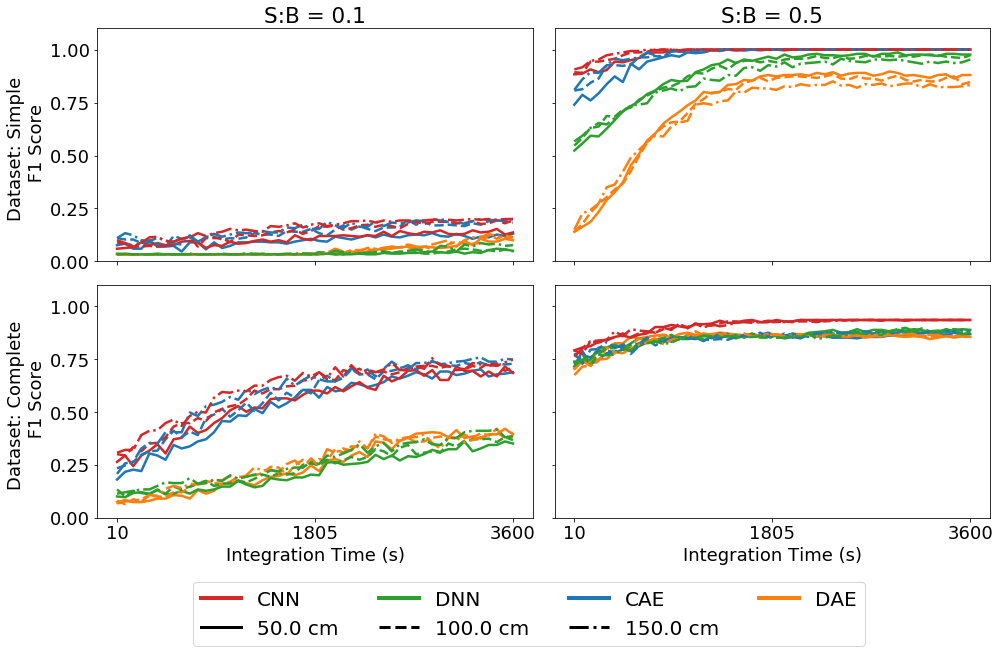
\includegraphics[width=1.0\linewidth]{images/sim-generalization-height}
	\caption{F1 score dependence Height generalization.}
	\label{fig:sim-generalization-height}
\end{figure}


\subsection{Generalization Performance Dependence on Source-Detector Distance}

In this section we analyze how each model's F1 score depends on changes in source-detector distance. This tests if each model is sensitive to larger changes in the Compton continuum compared to those associated with changes in source-detector height. An example of these changes can be seen in Figure \ref{fig:sim_spectra_distance_comparison}.

As seen in Figure \ref{fig:sim-generalization-dist}, we observe similar trends seen in the source-detector height generalization such as superior performance of the convolutional models and the poor simple DAE encoding. Changing the source-detector distance changes performance more noticeably compared to changes in standoff distance.

This change is especially noticeable for the shorter standoff distance of 50 cm. At this distance, the peak-to-total ratio increases significantly. The rise in peak-to-total ratio emphasizes the peak information while reducing the Compton continuum's contribution. Each model's F1 score is higher when benchmarked against lower signal-to-background spectra due to the increased photopeak information. This trend does not continue in the higher signal-to-background ratio spectra. At the higher ratio, each model's worst F1 score is achieved when benchmarked against spectra simulated with a 50 cm distance. As seen in Figure \ref{fig:sim_spectra_distance_comparison}, spectra simulated at a distance of 50 cm have a much different shape than spectra simulated at 175 cm or 300 cm. The simple models only trained with source-detector distances of 175 cm, making identifications for 50 cm spectra very difficult. The complete models trained using each simulated distance. The models could achieve a lower cost function error if they selectively updated weights associated with the 175 cm and 300 cm spectra because they were similar. This explains each complete model's reduced performance when identifying spectra simulated at 50 cm. 

This result also shows that each model is sensitive to a spectrum's photopeaks and shape of it's continuum. If the models were only sensitive to photopeaks, spectra simulated at a distance of 50 cm would have performed best in all cases due to the increased peak-to-total ratio.


\begin{figure}[H]
	\centering
	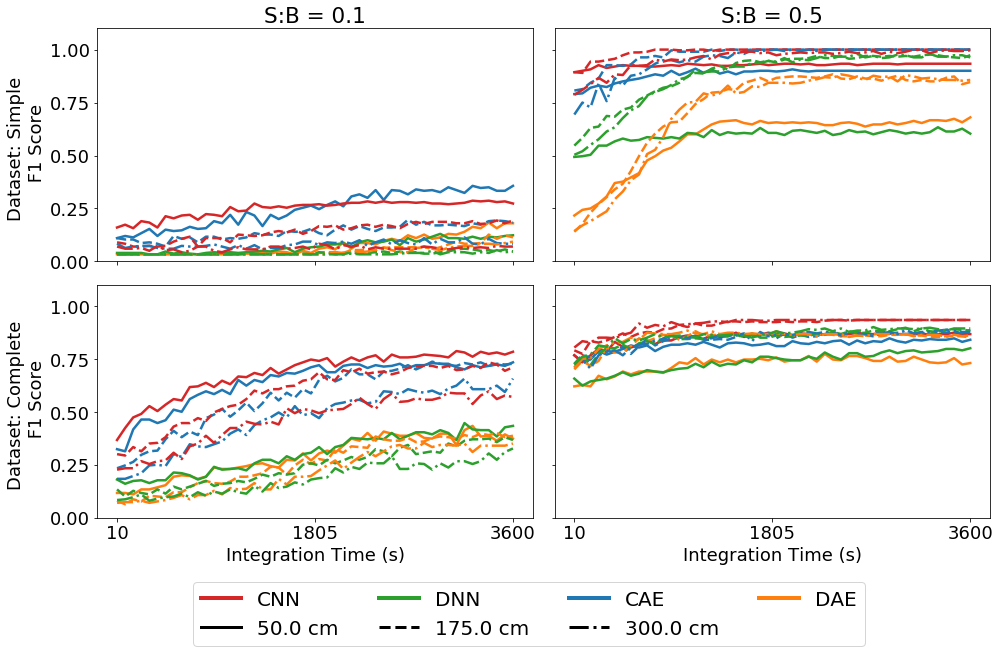
\includegraphics[width=1.0\linewidth]{images/sim-generalization-dist}
	\caption{Distance generalization.}
	\label{fig:sim-generalization-dist}
\end{figure}



\subsection{Generalization Dependence on Resolution}

In this section we analyze how each model's F1 score depends on changes in detector resolution. An example of these changes can be seen in Figure \ref{fig:sim-generalization-fwhm}. Changes in resolution do not significantly impact performance of the models. General trends are similar to distance and height generalization. 

\begin{figure}[H]
	\centering
	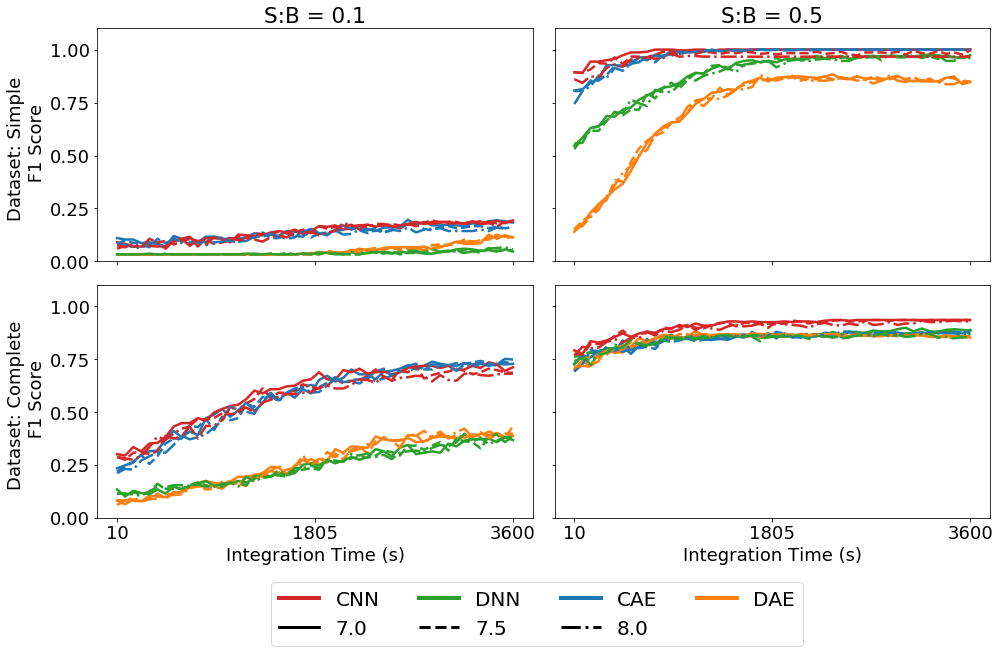
\includegraphics[width=1.0\linewidth]{images/sim-generalization-fwhm}
	\caption{Resolutions generalization.}
	\label{fig:sim-generalization-fwhm}
\end{figure}


\subsection{Generalization Dependence on Shielding.}

In this section we analyze how each model's F1 score depends on changes in shielding. Spectra were simulated with iron thicknesses that shield 40\%, 60\%, and 80\% of the intensity of a 200 keV gamma-ray.

As seen previously, simple models do not generalize to the lower signal-to-background spectra. Simple models, which only use unshielded and 20\% shielded templates, achieve F1 scores between 50\% and 75\% in higher signal-to-background spectra. This shows that simple models generalize to other shielding thicknesses in higher signal-to-background spectra. The simple CAE outperforms the CNN in spectra with each shielding thicknesses. This demonstrates that the CAE pretraining is useful for conditioning the convolutional weights for identification tasks. 

The complete models perform better in the low signal-to-background spectra. Both complete convolutional models perform comparatively and outperform the complete dense models. At 60\% and 80\% shielding the complete CAE outperformed the CNN in low signal-to-background spectra. This again shows the CAE pretraining boosting the CNN architecture's performance.

% The performance of each complete ANN decreases when identifying spectra with additional attenuation.


\begin{figure}[H]
	\centering
	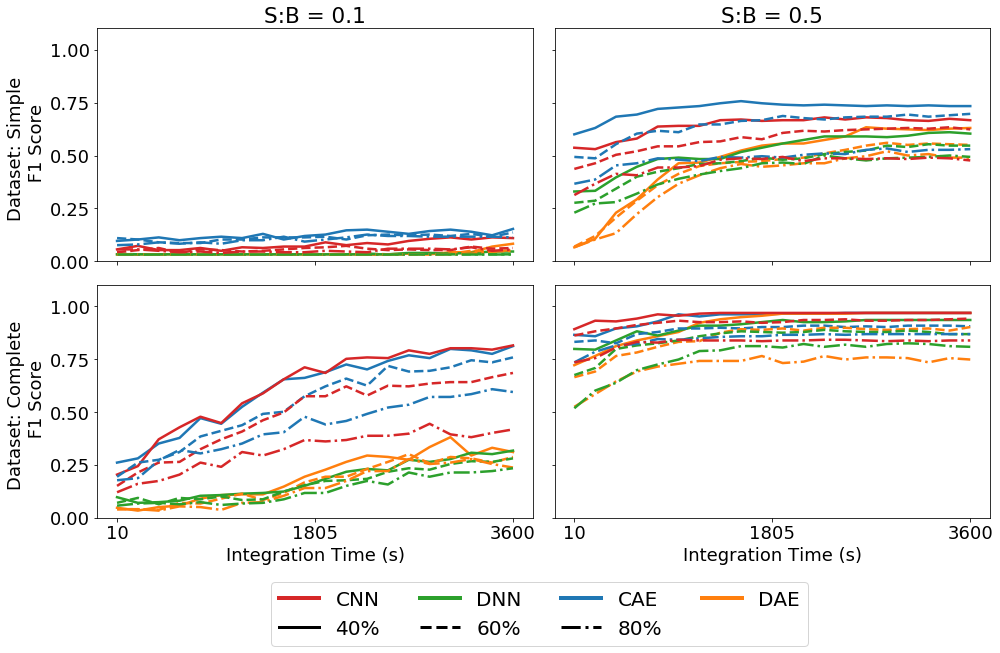
\includegraphics[width=1.0\linewidth]{images/sim-generalization-ironshield}
	\caption{Calibration gain generalization.}
	\label{fig:sim-generalization-ironshield}
\end{figure}

\subsection{Generalization Dependence on Gain}

In this section we analyze how each model's F1 score depends on changes in calibration. Spectra were simulated with relative calibration gains of 0.8, 1.0, and 1.2. These relative gain calibrations represent the range of calibrations expected due to temperatures expected when performing source interdiction. The 1.0 gain setting calibrates the 1024$^{th}$ channel of the spectrum to 3 MeV.

At the higher signal-to-background ratio, the simple convolutional models achieve F1 scores above 50\% for each gain setting except 0.8. Simple dense models achieve F1 scores between 30\% and 50\% for the same settings.


begin generalizing to the 1.2 relative gain while performing poorly on the 0.8 relative gain. The lower relative gain has the potential to push spectral features into the LLD, removing them from the input signal. Because the simple dataset parameters never obscure these features, the simple models cannot correctly identify spectra without them.

The complete models performed better with changing gain, but still struggled with the 0.8 relative gain for the reasons outline in the previous paragraph. Compared to other complete models, the complete CNN performed the best on each relative gain setting.

\begin{figure}[H]
	\centering
	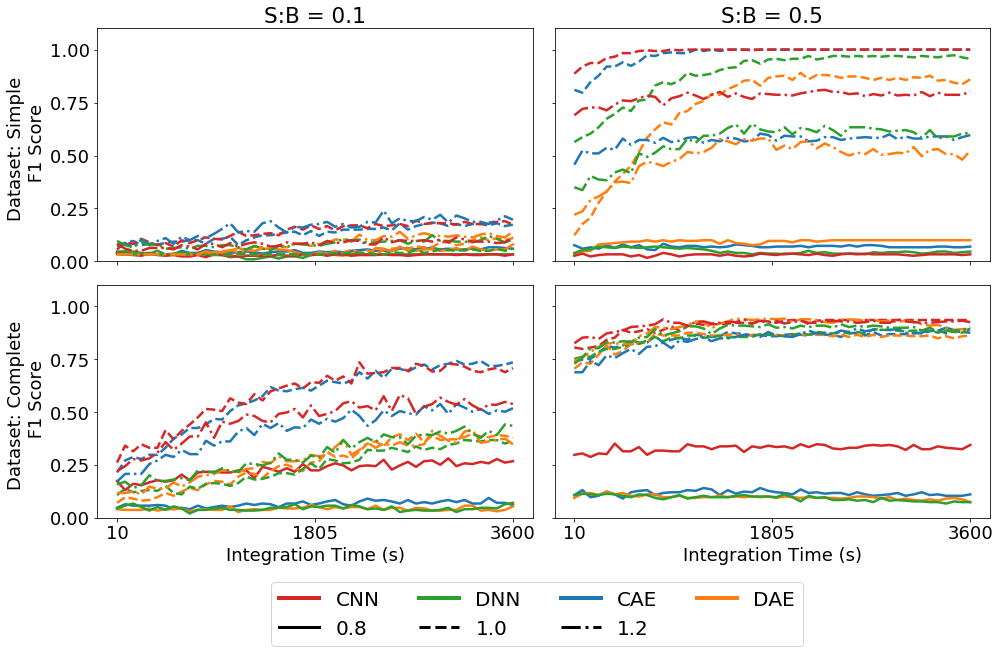
\includegraphics[width=1.0\linewidth]{images/sim-generalization-cal}
	\caption{Calibration gain generalization.}
	\label{fig:sim-generalization-cal}
\end{figure}




\section{Performance Identifying Measured Spectra}

In this section we investigate each ANN's performance when identifying real gamma-ray spectra with calibration settings and shielding possible in source interdiction activities. To measure performance, we observe how each model's posterior probability for each isotope changes over integration times ranging from 10 s to 10 mins. Sources included are $^{137}$Cs, $^{60}$Co, $^{133}$Ba, and $^{152}$Eu. $^{137}$Cs and $^{60}$Co are included because they have uncomplicated spectra, $^{137}$Cs with only one primary photopeak at 662 keV and $^{60}$Co with two photopeaks at 1173 and 1332 keV. These are also common industrial and medical sources which are important for source interdiction. $^{133}$Ba and $^{152}$Eu have more complicated spectra with many photopeaks. Photopeaks from $^{133}$Ba are all below 400 keV and the photopeaks from $^{152}$Eu range from 121 keV to 1213 keV \cite{bigbluebook}. $^{133}$Ba is included in these tests because it is a medical isotope and an often used surrogate for plutonium. $^{152}$Eu is included because it's large range of photopeak energies are uniquely effected by shielding and calibration changes. Shielding $^{152}$Eu can remove low-energy photopeaks while only slightly reducing higher-energy photopeaks. This presents a unique challenge for identification algorithms.

A diagram of the laboratory setup used for these measurements is shown in Figure \ref{fig:shielding_measurment_diagram}. The radioactive sources, 1 inch diameter by 1/8 inch thick plastic disks containing $\mu$Ci quantities of radioactive material, were measured on a wooden desk approximately one meter from the nearest wall to reduce environmental scatter. We used a 2x2 inch Ortec NaI detector to measure the sources. The source-detector distance, measured from the source disk's face to the detector's face, was adjusted to keep the signal-to-background ratio either 0.5 or 1.0. Blocks of shielding material were added for the measurements in Section \ref{real_shielding_performance}. Measurements in Section \ref{real_calibration_performance} used no shielding material. 

\begin{figure}[H]
	\centering
	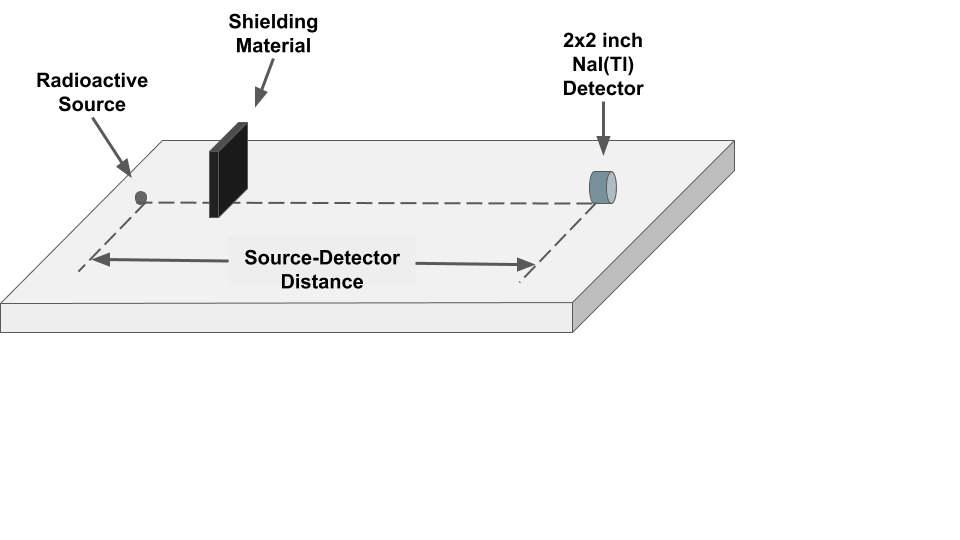
\includegraphics[trim=0 200 210 0,clip,width=0.9\linewidth]{images/shielding_measurment_diagram}
	\caption{Diagram of the laboratory setup used to measure radioactive sources.}
	\label{fig:shielding_measurment_diagram}
\end{figure}

For this section, we define a model's performance to be good when the posterior probability increases above 50 \% after 60 seconds. This measurement time is typical for source interdiction tasks. We also trigger an alarm when an isotopes posterior probability rises above 50\%. Plots in this section observe true positives, when the measured isotope's posterior probability exceed the 50\% threshold, and false negatives, when the measured isotope's posterior probability is below the 50\% threshold. For practical implementation, this threshold needs to be tuned for specific operational requirements. 


\subsection{Model Performance on Changing Voltage} \label{real_calibration_performance}

To test how well each model identified spectra with changing calibration, spectra were measured with different PMT voltages. PMT voltages included 720 V, 745 V, 770 V, and 795 V. The detector calibration of 770 V calibrated the detector's 1024$^{th}$ channel to 3 MeV. This gain setting was used as the reference calibration. Relative gain settings for the PMT voltages are measured with respect to the relative shift of the 662 keV photopeak. The source-detector distance of each source was adjusted so the ratio of counts per second from the source and background were 0.5 and 1.0. Example spectra measured at the experiment's time limits are shown for each isotope.

\subsubsection{$^{137}$Cs}

Example $^{137}$Cs spectra identified in this analysis are shown in Figure \ref{fig:realspectra-cal-cs137-spec}. The 662 keV photopeak is clearly visible even at a measurement time of 10 s. At a 10 s integration time, background peaks from $^{40}$K, at 1460 keV, and the thorium series, 2614 keV, are not visible. Without these peaks, it is very difficult to know the energy calibration of the detector.

\begin{figure}[H]
	\centering
	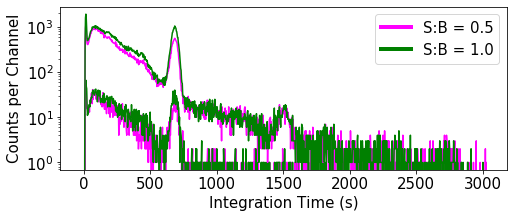
\includegraphics[width=0.85\linewidth]{images/realspectra-cal-cs137-spec}
	\caption{Example $^{137}$Cs measured with signal-to-background ratios of 0.5 and 1.0. The lower and higher count spectra use a measurement times of 10 s and 300 s respectively.}
	\label{fig:realspectra-cal-cs137-spec}
\end{figure}

Figure \ref{fig:realspectra-cal-cs137} demonstrates the effect of measurement time on each model's posterior probability for $^{137}$Cs. As time increases, the simple DNN and DAE monotonically increase their probabilities for $^{137}$Cs measured with the default gain. These probabilities approach an asymptote in the higher signal-to-background spectra. The simple CNN jumps to 100\% posterior probability for default gain spectra. Complete models demonstrate more monotonic performance for a wider range of gain settings. Monotonic increases in posterior probability are desirable for isotope identification algorithms because they are more easily interpreted by an unskilled user.

\begin{figure}[H]
	\centering
	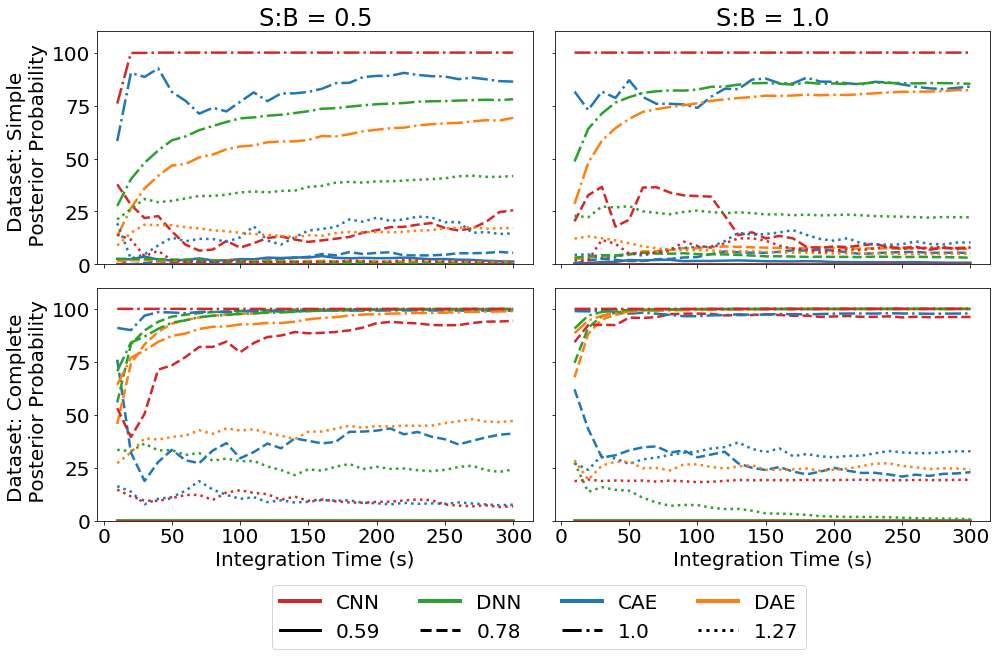
\includegraphics[width=1.0\linewidth]{images/realspectra-cal-cs137}
	\caption{Calibration gain generalization performance in real $^{137}$Cs spectra for the DNN, CNN with and without autoencoder pretraining.}
	\label{fig:realspectra-cal-cs137}
\end{figure}

Each ANN, except the simple DAE, identifies reference calibration spectra above the 50\% posterior probability threshold after 60 s of measurement. Simple ANNs fail to alarm on $^{137}$Cs spectra with other calibration settings. Complete ANNs, with the exception of the CAE, successfully alarm when identifying spectra with a relative gain of 1.0 and 0.78.

% This shows that even for an isotope with a single photopeak, ANN's cannot extrapolate outside of their 
Spectra with relative gains of 0.59 and 1.27 never raise a true positive alarm. These settings are too far outside of the training dataset's relative gain ranges, (0.8, 1.2), for correct identification. Correctly identifying $^{137}$Cs with a relative calibration of 1.27 are possible if the detection threshold is lowered, but this risks increasing the false positive rate. Spectra with a relative calibration of 0.59 move the 662 keV photopeak to 340 keV. As shown in Table \ref{table:cs137_precictions_60s}, ANNs mistakes $^{137}$Cs at this calibration for other isotopes with lower-energy photopeaks. The Simple CNN raises an incorrect alarm on $^{192}$Ir, which has it's largest photopeak at 316 keV. The complete CNN, DNN, and DAE also raise incorrect alarms. Both complete convolutional models predict the same isotope, $^{131}$I, which has a primary photopeak at 364 keV. Both dense models predict $^{239}$Pu.

\begin{table}[H]
	\centering
	\caption{ANN predictions of $^{137}$Cs spectra measured with a relative gain shift of 0.59. Spectra were measured with a signal-to-background ratio of 1.0 for 60 s. Incorrect alarms are bolded.}
	\label{table:cs137_precictions_60s}
	\begin{tabular}{lllll}
		\hline
		 & \multicolumn{4}{l}{\textbf{Simple}} \\
		 & \textbf{CNN} & \textbf{DNN} & \textbf{CAE} & \textbf{DAE} \\ \hline
		Prediction & \textbf{$^{192}$Ir} & $^{177m}$Lu &  $^{75}$Se  & $^{67}$Ga \\
		Probability & \textbf{80} & 33 & 41 & 33 \\ \hline \\ \\
		
		\hline
		Model & \multicolumn{4}{l}{\textbf{Complete}} \\
		& \textbf{CNN} & \textbf{DNN} & \textbf{CAE} & \textbf{DAE} \\ \hline
		Prediction  & \textbf{$^{131}$I} & \textbf{$^{239}$Pu} & $^{131}$I & \textbf{$^{239}$Pu}  \\ 
		Probability & \textbf{100} & \textbf{70} & 40 & \textbf{61} \\ \hline
	\end{tabular}
\end{table}


Even for isotopes with a single photopeak, Including a wide range of calibrations in a ANNs training dataset is necessary for good performance when identifying measured spectra.


\subsubsection{$^{60}$Co}

As seen in Figure \ref{fig:realspectra-cal-co60-spec}, the 1173 keV and 1332 keV photopeaks from $^{60}$Co spectra measured at 10 s each have a maximum number of counts less than 100. This is around a factor of two less than the maximum photopeak counts in the $^{137}$Cs spectra shown in the previous section. This amplifies the effects of Poisson noise on the $^{60}$Co spectra when compared to the $^{137}$Cs spectra.

\begin{figure}[H]
	\centering
	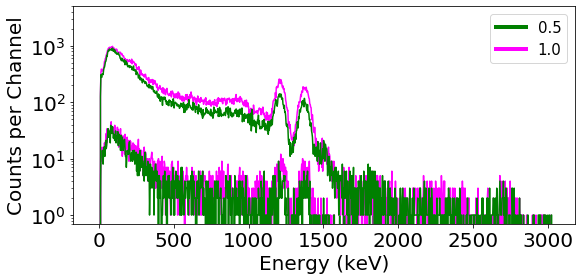
\includegraphics[width=0.85\linewidth]{images/realspectra-cal-co60-spec}
	\caption{Example $^{60}$Co spectra measured with signal-to-background ratios of 0.5 and 1.0. The lower and higher count spectra use a measurement times of 10 s and 300 s respectively.}
	\label{fig:realspectra-cal-co60-spec}
\end{figure}

Figure \ref{fig:realspectra-cal-co60} shows that monotonic behavior is observed in more $^{60}$Co identifications in a wider range of calibrations than observed for $^{137}$Cs. Similar to identifications for $^{137}$Cs, shown in Figure \ref{fig:realspectra-cal-cs137}, the convolutional models exhibited more erratic behavior than dense models.

\begin{figure}[H]
	\centering
	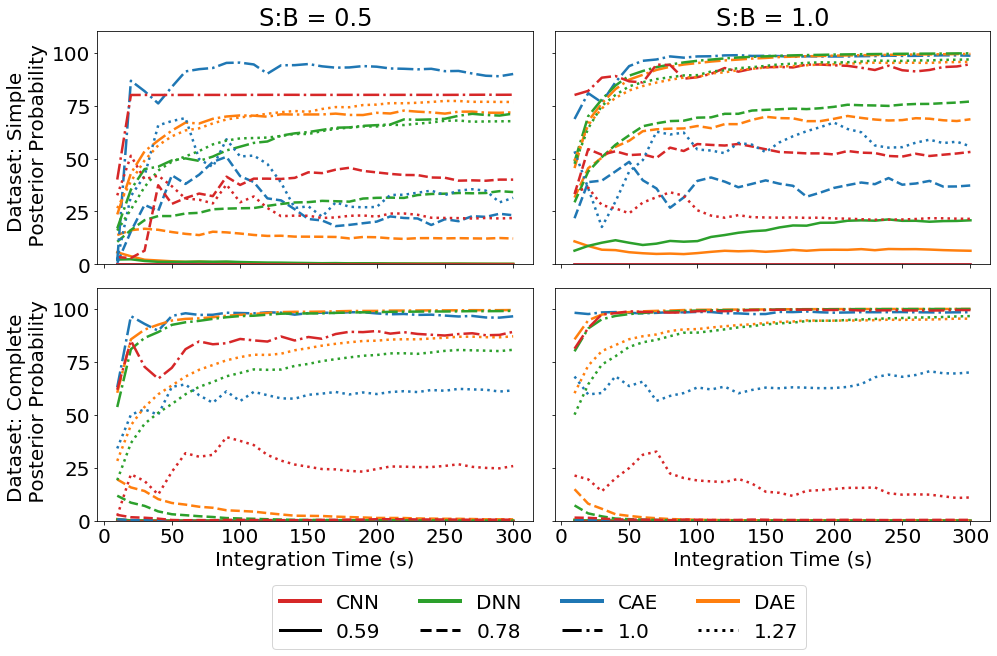
\includegraphics[width=1.0\linewidth]{images/realspectra-cal-co60}
	\caption{Calibration gain generalization performance in real $^{60}$Co spectra for the DNN, CNN with and without autoencoder pretraining.}
	\label{fig:realspectra-cal-co60}
\end{figure}

Simple ANNs correctly alarm on $^{60}$Co spectra measured using the default gain. This effect is also seen in the $^{137}$Cs identifications. Unlike identifications in $^{137}$Cs, both simple dense ANNs correctly alarm on the gain setting of 1.27. This shows that dense networks are more flexible when identifying spectra with parameters outside of their training set. Convolutional models may develop feature extraction mechanisms that are more prone to overtraining than dense models. Simple dense ANNs outperforming simple convolutional ANNs is also shown when identifying spectra measured with the higher signal-to-background ratio. Simple dense ANNs correctly alarm on spectra with all gain settings except 0.59.

Complete ANNs fail to alarm on spectra with a relative gain setting of 0.78. ANNs predict these spectra to be $^{238}$U with posterior probabilities above 98\%. The $^{238}$U spectrum is characterized by photopeaks at 93 keV, 766 keV, and 1001 keV. With sufficient shielding, the 93 keV photopeak is completely attenuated, leaving a two photopeaks. These photopeaks are have an energy similar to the photopeaks from $^{60}$Co. By including shielded $^{238}$U spectra in the complete training dataset, we introduced spectra similar to $^{60}$Co. 


\subsubsection{$^{133}$Ba}

$^{133}$Ba spectra are shown in Figure \ref{fig:realspectra-cal-ba133-spec}. Spectra measured for 10 s have features and photopeaks difficult to identify by eye. Due to a measurement error, $^{133}$Ba spectra measured at a signal-to-background ratio of 0.5 with a relative gain of 1.27 were lost. Spectra measured with this setting are replaced by spectra measured with a signal-to-background ratio of 0.5 and relative gain of 1.0 recalibrated to match a gain of 1.27.

\begin{figure}[H]
	\centering
	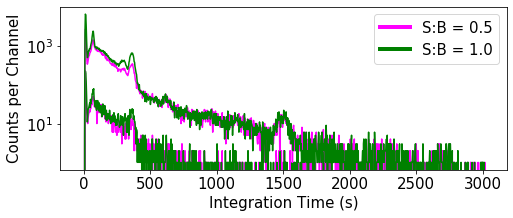
\includegraphics[width=0.85\linewidth]{images/realspectra-cal-ba133-spec}
	\caption{Example $^{133}$Ba spectra measured with signal-to-background ratios of 0.5 and 1.0. The lower and higher count spectra use a measurement times of 10 s and 300 s respectively.}
	\label{fig:realspectra-cal-ba133-spec}
\end{figure}

In most cases, dense models failed to achieve posterior probabilities above 20\% when identifying $^{133}$Ba spectra. Only the simple CAE with a source-to-background ratio of 1.0 alarmed after 120 s measurement time. The simple CAE only correctly identifies spectra measured using the default calibration. 

Only the complete CNN successfully alarms on $^{133}$Ba with a signal-to-background ratio of 0.5. Both convolutional models 

This shows that despite their erratic predictions, convolutional models may be necessary when identifying spectra similar to $^{133}$Ba. Adding relative gain settings using a finer sampling on the range (0.8, 1.2) may be necessary to consistently identify $^{133}$Ba spectra.


\begin{figure}[H]
	\centering
	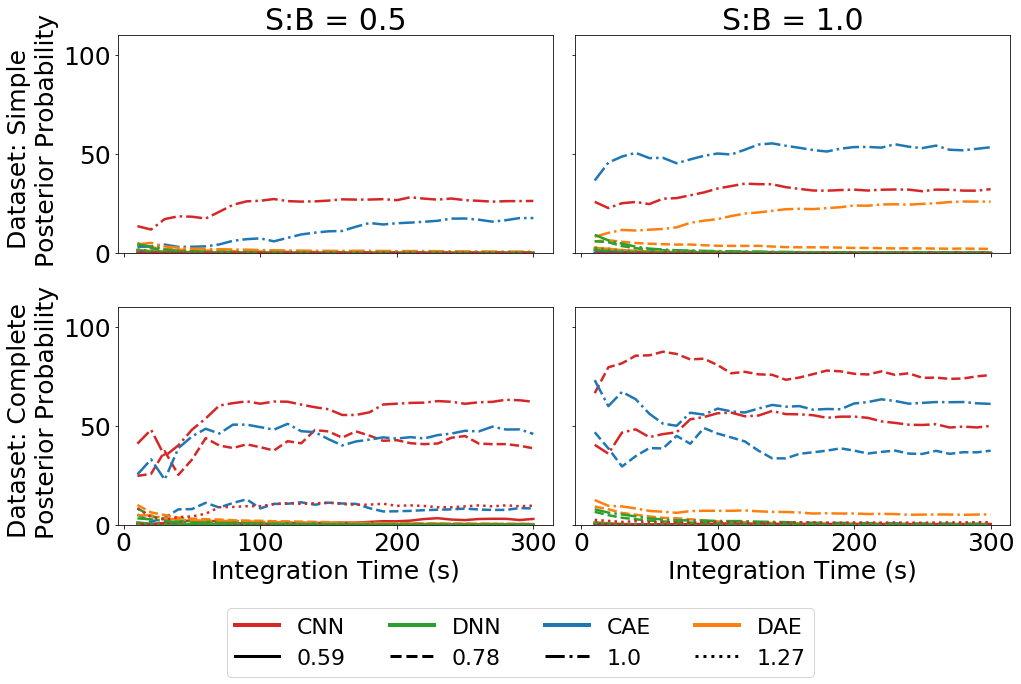
\includegraphics[width=1.0\linewidth]{images/realspectra-cal-ba133}
	\caption{Calibration gain generalization performance in real $^{133}$Ba spectra for the DNN, CNN with and without autoencoder pretraining.}
	\label{fig:realspectra-cal-ba133}
\end{figure}


\subsubsection{$^{152}$Eu}

Spectra of $^{152}$Eu are shown in Figure \ref{fig:realspectra-cal-eu152-spec}. $^{152}$Eu emits photons with a wide range of energies. 

\begin{figure}[H]
	\centering
	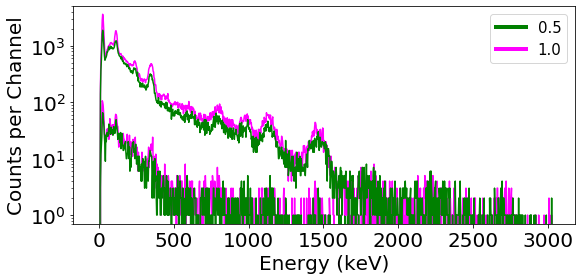
\includegraphics[width=0.85\linewidth]{images/realspectra-cal-eu152-spec}
	\caption{Example $^{152}$Eu spectra measured with signal-to-background ratios of 0.5 and 1.0. The lower and higher count spectra use a measurement times of 10 s and 300 s respectively.}
	\label{fig:realspectra-cal-eu152-spec}
\end{figure}

Higher signal-to-noise $^{152}$Eu is identified correctly with a 60 s measurement 

% Figures in \ref{fig:realspectra-cal-eu152} show performance when identifying $^{152}$Eu. For the first time, convolutional architectures did not outperform the dense models. This performance change only occurred in the simple dataset. As explained above, because of the lack of spectral variety in the simple dataset, generalization to real spectra is more difficult. $^{152}$Eu has many more identifiable photopeaks in a larger range of energies compared to $^{133}$Ba. Because of this, using the channel-based approach (dense architectures) would lead to better performance over approaches that use a form of feature extraction.


% The improvement in the convolutional models for $^{152}$Eu identification occurs when more spectral variety is available in the complete dataset. With the complete dataset, all gain settings except 0.59 are identified with high posterior probability above 100 seconds of integration time. 


\begin{figure}[H]
	\centering
	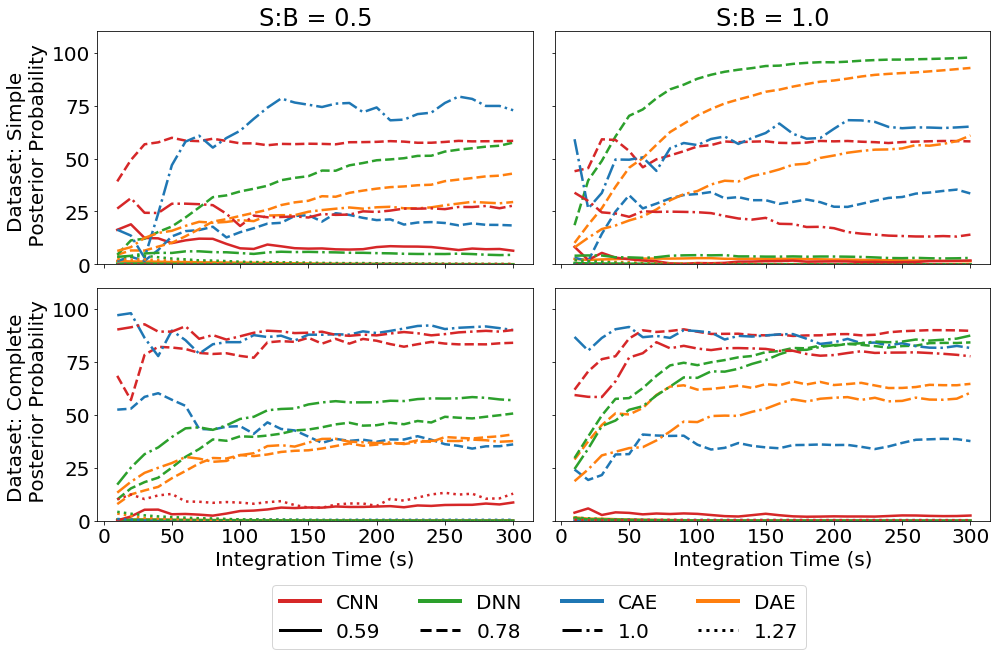
\includegraphics[width=1.0\linewidth]{images/realspectra-cal-eu152}
	\caption{Calibration gain generalization performance in real $^{152}$Eu spectra for the DNN, CNN with and without autoencoder pretraining.}
	\label{fig:realspectra-cal-eu152}
\end{figure}

\subsection{Model Performance with Respect to Shielding} \label{real_shielding_performance}

To investigate the identification performance of each ANN with increased shielding thicknesses, sources were shielded with increasingly thick iron or aluminum blocks and measured. For each measurement, the source-detector distance was adjusted so the ratio of counts per second measured by the detector was equal to the counts per second from background. Each spectrum was measured using the default detector PMT calibration of 770 V. 

\subsubsection{$^{137}$Cs}


Figure \ref{fig:shielded_cs137} shows that shielding affects the $^{137}$Cs spectrum by reducing the 662 keV photopeak's peak-to-total ratio. Shielding does not visibly impact the shape of Compton continuum. 

\begin{figure}[H]
	\centering
	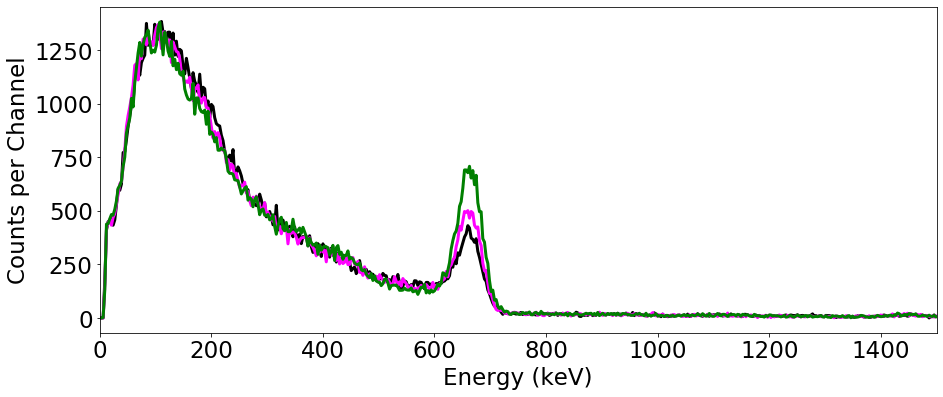
\includegraphics[width=0.8\linewidth]{images/shielded_cs137}
	\caption{Spectra of $^{137}$Cs shielded with increasing amounts of iron measured for 60 s.}
	\label{fig:shielded_cs137}
\end{figure}

As seen in Figure \ref{fig:iron_cs137}, all simple and complete models correctly alarm on each shielded $^{137}$Cs isotope. Shielding impacts the simple dense models' performance more than the convolutional models. This reduction in performance is demonstrated by a reduced posterior probability. The DAE outperforms the DNN, achieving a higher posterior probability for each shielding thickness after 50 s. This demonstrates that the dense pretraining improved the dense model's performance.

Each complete model achieves a posterior probability above 90\% for all measured times and shielding thicknesses. This shows that the additional parameters in the complete training dataset boost performance in trained ANNs when identifying shielded isotopes.

\begin{figure}[H]
	\centering
	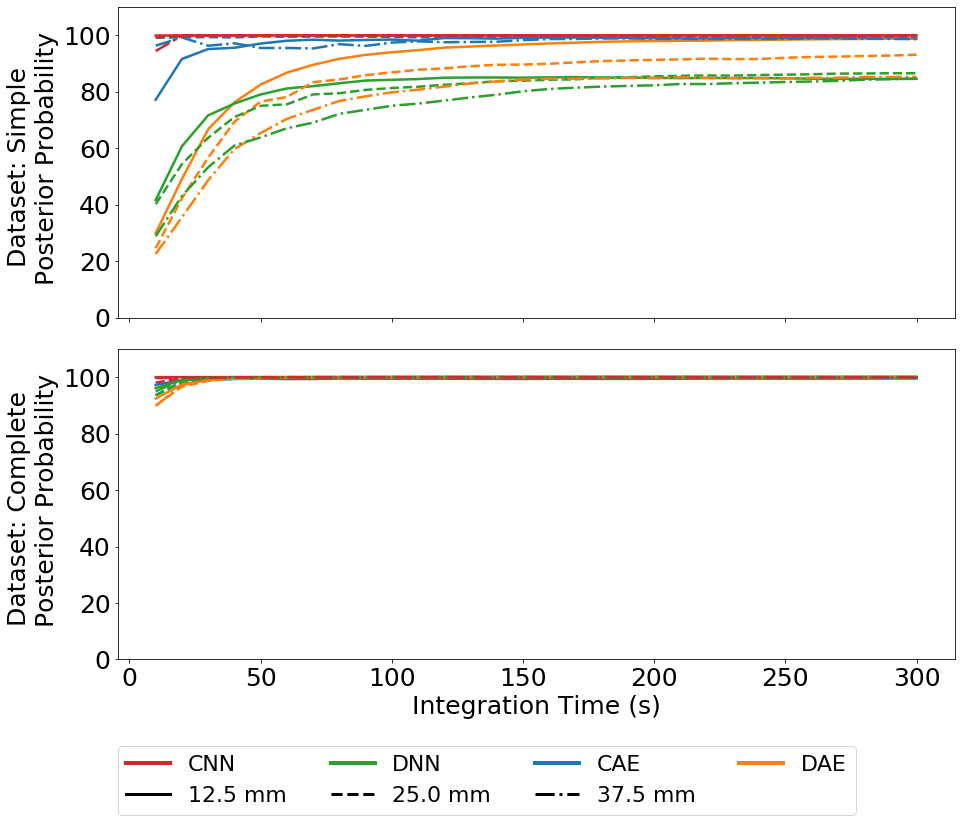
\includegraphics[width=0.8\linewidth]{images/iron_cs137}
	\caption{Shielding generalization performance in real $^{137}$Cs spectra.}
	\label{fig:iron_cs137}
\end{figure}




\subsubsection{$^{60}$Co}

As shown in Figure \ref{fig:shielded_co60}, the effect of shielding is not visibly significant in $^{60}$Co spectra. The 1173 keV and 1332 keV photopeaks from $^{60}$Co are attenuated less than the 662 keV photopeak from $^{137}$Cs. Shielding only slightly decreases the area of the $^{60}$Co photopeaks.

\begin{figure}[H]
	\centering
	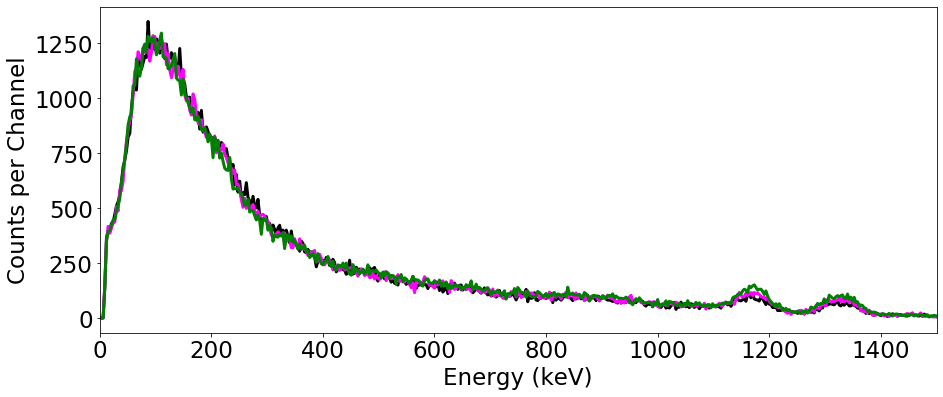
\includegraphics[width=0.8\linewidth]{images/shielded_co60}	\caption{Spectra of $^{60}$Co shielded with increasing amounts of iron measured for 60 s.}
	\label{fig:shielded_co60}
\end{figure}

As seen in Figure \ref{fig:iron_co60}, each simple convolutional model successfully alarms on each shielded  $^{60}$Co spectrum. In particular, the CAE identifies each shielded $^{60}$Co spectrum with a near 100\% posterior probability after 20 s. This demonstrates that the natural feature extraction capabilities of convolutional models work well when identifying simple spectra with shielding amounts not included in their training dataset. This also shows that using autoencoder pretraining increases the convolutional model's performance.

\begin{figure}[H]
	\centering
	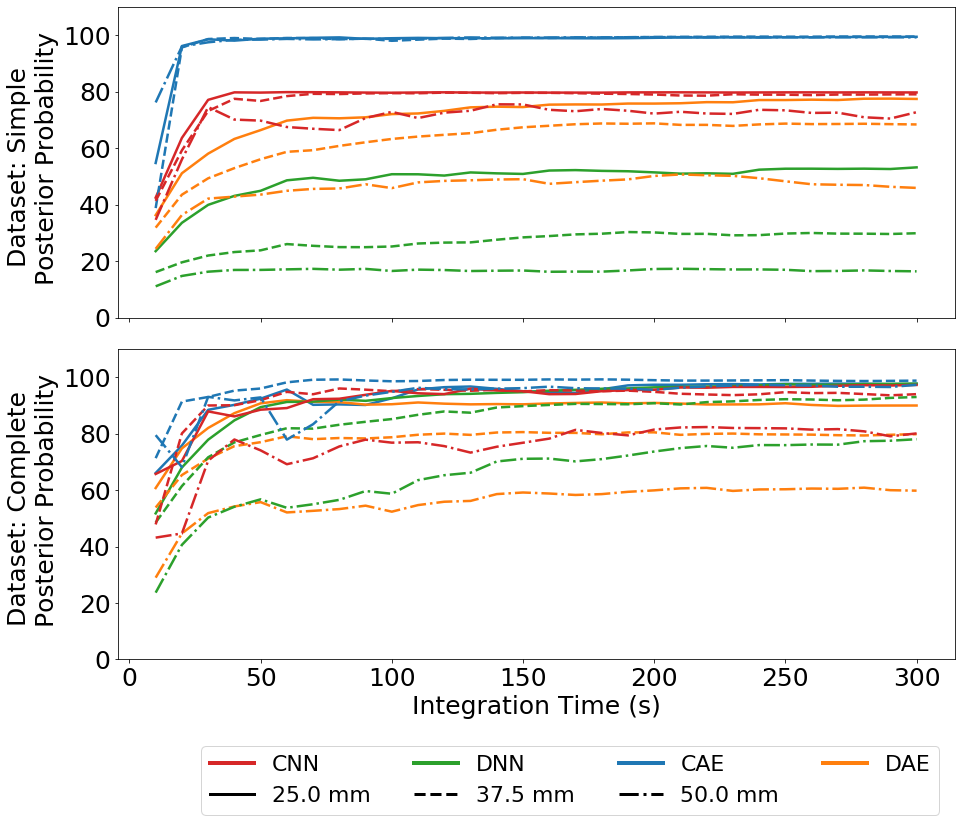
\includegraphics[width=0.8\linewidth]{images/iron_co60}	\caption{Shielding generalization performance in real $^{60}$Co spectra.}
	\label{fig:iron_co60}
\end{figure}

Shielding has a larger detrimental impact on simple dense ANNs compared to simple convolutional ANNs. Despite a clear photopeak at 662 keV, only the DAE successfully alarms on $^{60}$Co shielded with the two thinnest iron blocks. As with the convolutional model, this result shows that dense models visibly improve with autoencoder pretraining. The poor performance of the simple dense models is attributed to overtraining on the single $^{60}$Co example in the training dataset. 

Each model's performance improves when trained on the complete dataset. All complete ANNs successfully alarm on spectra measured with each shielding thickness. Both complete convolutional ANNs have comparable performance. Similar to the simple models, complete dense ANNs achieve posterior probabilities less than the comple convolutional ANNs.

\subsubsection{$^{133}$Ba}

Due to the relatively low gamma-ray energies of $^{133}$Ba compared to the other spectra in this section, aluminum with thicknesses of 6.56 mm, 25.5 mm, and 51.0 mm were used as the shielding material. Characteristic $^{133}$Ba photons have relatively low energy - particularly the photopeaks at 31 and 81 keV. As seen in Figure \ref{fig:shielded_ba133}, shielding significantly distorts the spectrum at these energies.

\begin{figure}[H]
	\centering
	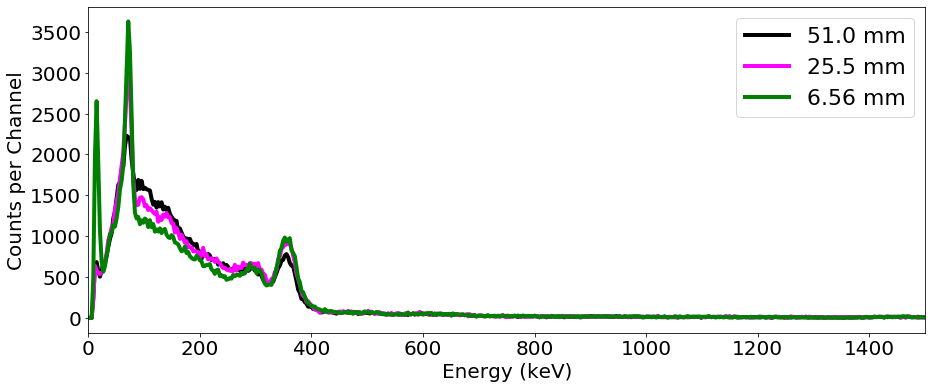
\includegraphics[width=0.8\linewidth]{images/shielded_ba133}
	\caption{Spectra of $^{133}$Ba shielded with increasing amounts of aluminum measured for 60 s.}
	\label{fig:shielded_ba133}
\end{figure}

As seen in Figure \ref{fig:alum_ba133}, all simple ANNs, except the simple CAE, fail to correctly alarm when identifying shielded $^{133}$Ba spectra. The simple CAE correctly alarms only when identifying $^{133}$Ba with the thinnest shielding. This shows that the models trained on the simple dataset will perform poorly when measuring shielded spectra visibly distorted by shielding material.

\begin{figure}[H]
	\centering
	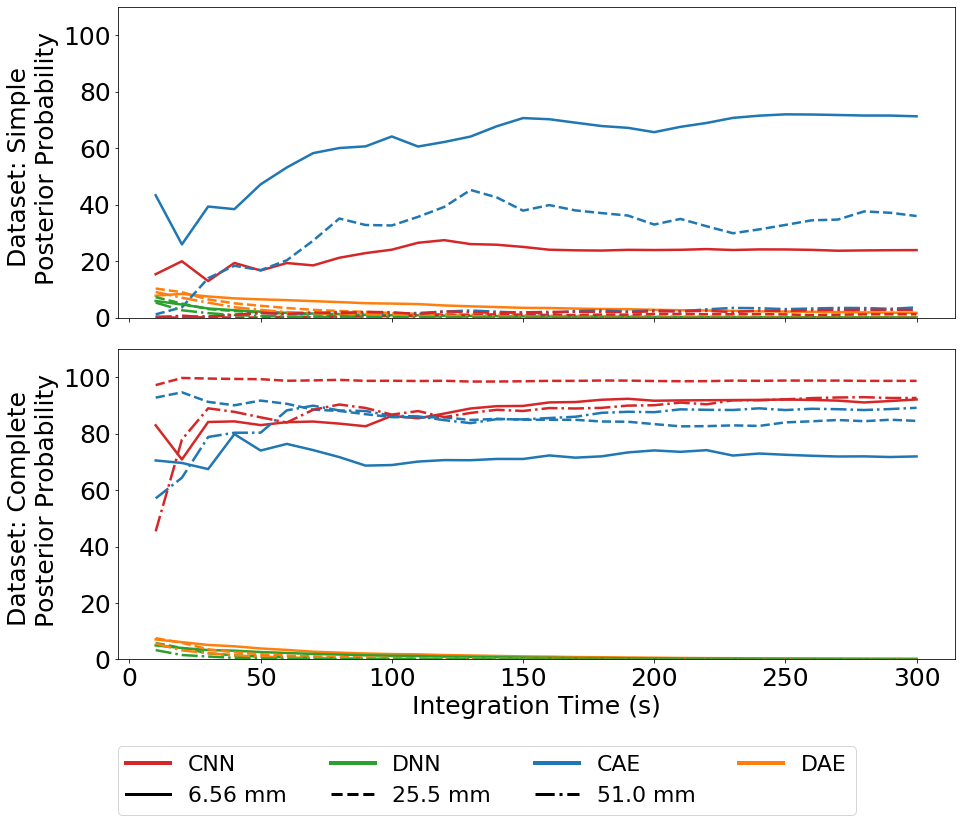
\includegraphics[width=0.8\linewidth]{images/alum_ba133}	\caption{Shielding generalization performance in real $^{133}$Ba spectra.}
	\label{fig:alum_ba133}
\end{figure}

Each complete convolutional models perform very well on all shielded $^{133}$Ba spectra. Each model successfully alarms after 20 s. Dense models perform poorly, incorrectly alarming on $^{131}$I in spectra with the thinnest shielding and $^{51}$Cr in spectra with thicker shielding material. The largest photopeak from $^{131}$I is located at 364 keV and the single photopeak from $^{51}$Cr is located at 320 keV. The complete dense ANNs poor performance when identifying shielded $^{133}$Ba indicates that they are poor choices for differentiating spectra with low-energy photopeaks. This is concerning because medical sources, plutonium, and uranium all have characteristic photopeaks below 400 keV. These low-energy photopeak sources are particularly important to identify and differentiate for source interdiction.


\subsubsection{$^{152}$Eu}

As seen in Figure \ref{fig:shielded_eu152}, $^{152}$Eu has many photopeaks spread across a large range of energies. As with $^{133}$Ba, higher-energy photopeaks (like those at 779 keV, 963 keV, 1086 keV, 1112 keV, and 1408 keV) are attenuated less than lower-energy photopeaks (like those at 122 keV and 344 keV).

\begin{figure}[H]
	\centering
	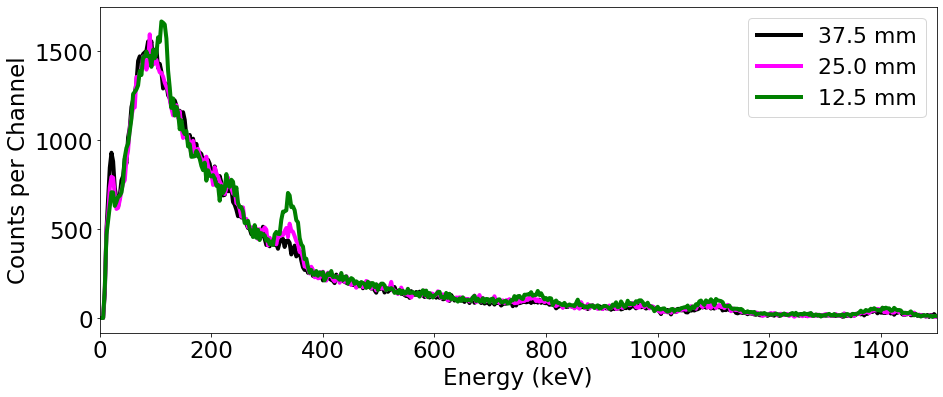
\includegraphics[width=0.8\linewidth]{images/shielded_eu152}
	\caption{Spectra of $^{152}$Eu shielded with increasing amounts of iron measured for 60 s.}
	\label{fig:shielded_eu152}
\end{figure}

Identification results for shielded $^{152}$Eu are shown in Figure \ref{fig:iron_eu152}. Similar to identifications in shielded $^{133}$Ba, the simple CAE correctly alarms on $^{152}$Eu spectra shielded with the two thinnest shielding materials. In addition to this, the simple DNN correctly alarms on spectra measured with the lightest shielding thickness.

\begin{figure}[H]
	\centering
	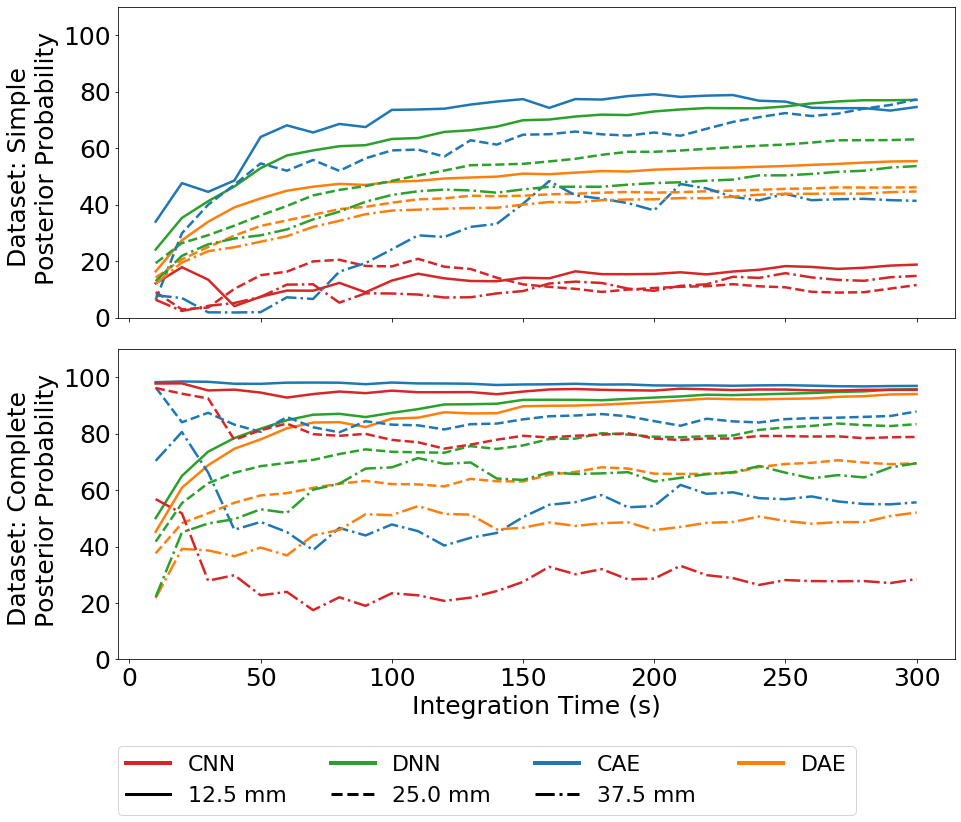
\includegraphics[width=0.8\linewidth]{images/iron_eu152}
	\caption{Shielding generalization performance in real $^{152}$Eu spectra.}
	\label{fig:iron_eu152}
\end{figure}

All complete models successfully alarm on $^{152}$Eu spectra shielded with the two thinnest blocks of iron. Both $^{152}$Eu and $^{133}$Ba have a large number of photopeaks compared to $^{60}$Co and $^{137}$Cs. Despite the large number of photopeaks, ANNs correctly identify $^{152}$Eu more often than $^{133}$Ba. The difference between these two isotopes is that $^{152}$Eu has a unique set of photopeaks relative to the library of training isotopes. The unique set of photopeaks in a wide range of energies make identification easier for the ANNs. As previously discussed, $^{133}$Ba possesses a large number of photopeaks in the lower-energy region shared by other isotopes' photopeaks. To improve identification of these important low-energy isotopes, additional examples of them need to be included in each ANN's training dataset.

\section{Comparison with Peak-Based Bayesian Classifier}

In this section we compare our trained ANNs to the performance of a peak-based Bayesian classifier created in Dr. Jacob Stinnett's PhD dissertation \cite{stinnett2016}. The peak-based classifier extracts photopeak locations and areas using a wavelet transform. These features are then used in a Bayesian classifier to produce posterior probabilities for a library of ANSI N42-34-2006 standard isotopes. Following the same procedure as Dr. Stinnett, we simulated the same sources using the same 20 s measurement time. Simulated sources were modeled after measured sources that are included in the AIP. The sources include: $^{241}$Am, $^{133}$Ba, $^{57}$Co, $^{60}$Co, $^{137}$Cs, $^{152}$Eu, $^{67}$Ga, $^{125}$I, $^{131}$I, $^{192}$Ir, $^{40}$K, $^{226}$Ra, $^{99m}$Tc, $^{201}$Tl, $^{233}$U, high enriched uranium (HEU), and weapons grade plutonium (WGPu). HEU was defined to be identified correctly if the ANN's highest posterior probability output identified $^{235}$U. WGPu was defined to be identified correctly if the ANN identified either $^{241}$Am, $^{239}$Pu, or $^{240}$Pu. Each of these isotopes are present in WGPu spectra.

F1 scores for trained ANNs and the peak-based Bayesian classifier are shown in Table \ref{table:jacob_compare}. As seen in Table \ref{table:jacob_compare}, each ANN, except the simple autoencoders, outperform the Bayesian classifier. Complete ANNs match or outperform their simple counterparts. The complete DNN achieves the highest F1 score. 

\begin{table}[H]
	\centering
	\caption{F1 scores from the Bayesian classifier and ANNs. The highest F1 scores are shown in bold.}
	\label{table:jacob_compare}
	\begin{tabular}{ll}
		\hline
		\textbf{Model} &  \textbf{F1 Score [\%]} \\ \hline
		Bayesian classifier & 71.47 \\ 
		Simple CNN & 78.79 \\ 
		Simple DNN & 72.73 \\ 
		Simple CAE & 66.67 \\ 		
		Simple DAE & 60.61 \\ 
		Complete CNN & 78.79 \\ 
		Complete DNN & \textbf{84.85} \\ 
		Complete CAE & 78.79 \\ 
		Complete DAE & 78.79 \\ \hline
	\end{tabular}
\end{table}

Incorrect identifications are shown in Table \ref{table:anns_incorrect}. Incorrect identifications typically involve isotopes that present only a few low energy photopeaks. Examples of this are $^{125}$I classified as $^{241}$Am; $^{241}$Am classified as $^{204}$Tl and $^{133}$Xe; $^{99m}$Tc classified as $^{131}$I; and $^{57}$Co classified as $^{99m}$Tc. The Bayesian classifier also experienced issues identifying isotopes in this category, particularly $^{125}$I. The Bayesian classifier also misidentified $^{233}$U, likely due to contamination from $^{232}$U.

\begin{table}[H]
	\centering
	\caption{Isotopes incorrectly classified by the ANNs. Entries with dashes indicate a correct identification.}
	\label{table:anns_incorrect}
	\begin{tabular}{lllll}
		\hline
		& \multicolumn{4}{l}{\textbf{Training Dataset - Simple}} \\
		\textbf{True Label} & \textbf{CNN} & \textbf{DNN} & \textbf{CAE} & \textbf{DAE} \\ \hline
		$^{125}$I & $^{241}$Am & $^{241}$Am & $^{241}$Am & $^{241}$Am \\ 
		$^{233}$U & $^{137}$Cs & $^{226}$Ra & $^{57}$Co &  $^{226}$Ra  \\ 
		WGPu & - & $^{201}$Tl & $^{201}$Tl & $^{201}$Tl \\ 
		$^{241}$Am & - & $^{204}$Tl &- & $^{133}$Xe \\
		$^{40}$K & Background & $^{60}$Co & Background & $^{60}$Co \\
		$^{57}$Co & - & - & - & $^{60}$Co \\
		$^{99m}$Tc & $^{131}$I & $^{131}$I & $^{131}$I & $^{131}$I \\ \hline \\ \\
		
		\hline
		& \multicolumn{4}{l}{\textbf{Training Dataset - Complete}} \\
		\textbf{True Label} & \textbf{CNN} & \textbf{DNN} & \textbf{CAE} & \textbf{DAE} \\ \hline
		$^{125}$I & $^{241}$Am & $^{241}$Am & $^{241}$Am & $^{241}$Am  \\ 
		$^{233}$U & $^{99}$Mo & $^{137}$Cs & $^{153}$Sm &  $^{137}$Cs \\ 
		$^{235}$U & - & - &  $^{177m}$Lu  & - \\ 
		$^{241}$Am & $^{133}$Xe & - & - & - \\	
		$^{57}$Co & - & - & - & $^{99m}$Tc \\ \hline \\ \\
	\end{tabular}
\end{table}


\section{Chapter Discussion and Conclusion}

This chapter shows that CNNs trained on the complete dataset generalize very well to simulated and real gamma-ray spectra. When trained on the simple dataset CNNs often also perform well when identifying spectra outside the simple dataset's parameters, but struggle with real spectra. The autoencoders perform poorly in the simulated spectra, but generalize well to parameters outside the simple training set - particularly DAEs. There is also some evidence that CAEs generalize better to isotopes with predominately low energy photopeaks in real spectra. Occasionally, at the lower signal-to-background ratio, the DNN outperforms the CNN. Because the dense architecture is more suited to comparing counts in different regions, it should be more robust against changes in Compton continua as it compares counts in photopeak areas. Despite this, DNN's offer unpredictable performance. Due to the large number of inputs, the DNN's are likely overtraining to specific combinations of noise in the training datasets.




